%
% $RCSfile: ontology.tex,v $
%
% Copyright (c) 2001-2004. Christian Heller. All rights reserved.
%
% Permission is granted to copy, distribute and/or modify this document
% under the terms of the GNU Free Documentation License, Version 1.1
% or any later version published by the Free Software Foundation;
% with no Invariant Sections, with no Front-Cover Texts and with no Back-Cover
% Texts. A copy of the license is included in the section entitled
% "GNU Free Documentation License".
%
% http://www.cybop.net
% - Cybernetics Oriented Programming -
%
% http://www.resmedicinae.org
% - Information in Medicine -
%
% @author Christian Heller <christian.heller@tuxtax.de>
% @author Jens Bohl <info@jens-bohl.de>
%

\section{Ontology}
\label{ontology_heading}

An ontology is a catalogue of types that are depending on each other in hierarchical
order. It is a formal specification concerning a particular objective. CYBOP
consists of three such ontologies:
\begin{itemize}
    \item{Basic Ontology}
    \item{Model Ontology}
    \item{System Ontology}
\end{itemize}

Figure \ref{model_ontology_figure} shows the model ontology. The layer super types
are {\tt Record}, {\tt Unit}, {\tt Heading} and {\tt Description}. These classes
are super types of all classes in a particular ontological level.\\
The right side shows a concrete implementation of the model ontology -- the
\emph{Electronic Health Record} \cite{openehr}. This data structure contains all
information concerning a particular patient. The figure shows {\tt Problem} types
in level {\tt Unit}. These consist of episodes containing instances of
{\tt PartialContact}. In level {\tt Heading}, the structural elements of a partial
contact can be found -- {\tt Subjective}, {\tt Objective}, {\tt Assessment} and
{\tt Plan}. Therapeutical issues are placed in level {\tt Description} -- such as
{\tt Medication} with particular dose.

\begin{figure}[ht]
    \begin{center}
       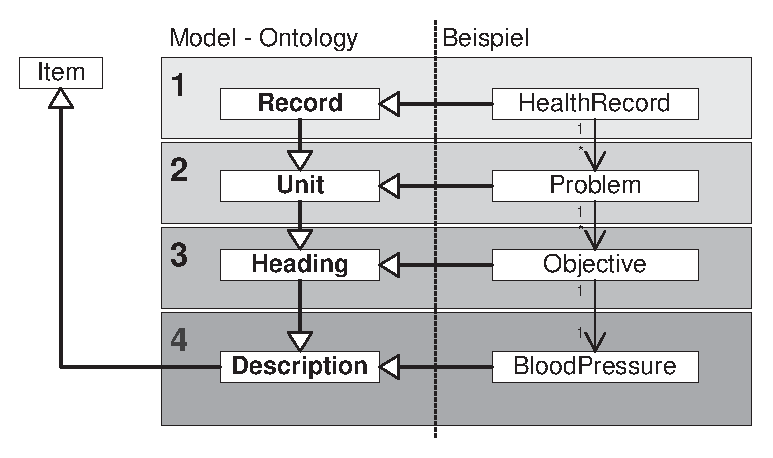
\includegraphics[scale=0.6]{eps/ModelOntologyUML.eps}
       \caption{Model Ontology}
       \label{model_ontology_figure}
    \end{center}
\end{figure}

As shown, the concept of ontology can be used to organize data structures in
a hierarchical order by defining logical layers with super types.

